\chapter{Background Literature}\label{chap:lit}
\begin{overview}
  A literature overview on model predictive control and controller constraints
  is presented in this chapter. Process operability is reviewed and the
  operability index -- used as the basis for constraint interaction -- is 
  defined. Finally, a summary of the mathematical techniques used is given.
\end{overview}

\section{Model Predictive Control}
Since its successful implementation in the petrochemical industry, model
predictive control (MPC) has gained widespread acceptance in the processing 
sector \citep[1]{maciejowskimpc}. This has led to the development of many 
commercial MPC packages such as DMCPlus (Aspentech), RMPCT (Honeywell),
Connoisseur (Invensys) and SMOC (Shell Global Solutions) \citep{qinbadgwell}.
\subsection{Control theory}
Model predictive control differs from other model based control techniques (such
 as Inverse Nyquist Array- and Internal Model Control) in its active use of 
predictions for future process outcomes \citep[137]{maciejowskifb}. In this 
context, MPC further distinquishes itself from other predictive control
techniques in its ability to accomodate constraints on inputs and outputs.

\citet[8]{maciejowskimpc} summarises the control methodology of MPC in four 
steps; Measure, Predict, Optimize/Calculate and Apply. Along with 
figure~\ref{fig:mpc:general} these steps are summarized below;
%TODO - add symbols to list
\begin{enumerate}
  \item Measure; the current outputs are measured and the error (deviation from
    the setpoint trajectory) is calculated.
  \item Predict; using the model, future outputs are calculated (over the 
    prediction horizon).
  \item Optimize/Calculate; control moves (over the control horizon) are now
    calculated to minimize the predicted deviation from the setpoint trajectory.
  \item Apply; only the first control move is implemented, whereafter this 
    procedure is restarted.
\end{enumerate}
\begin{figure}[htbp]
  \centering
  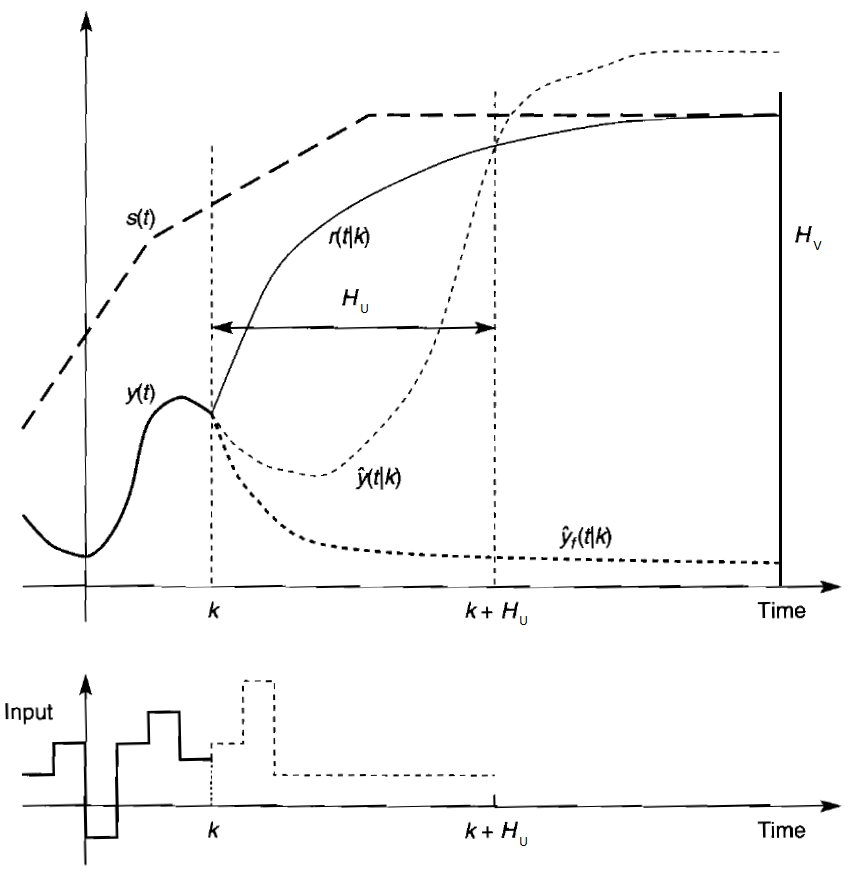
\includegraphics[width=\fullwidth]{graph/mpc_general}
  \caption[General MPC working]{General MPC working, showing predictions on both outputs and inputs}
  \label{fig:mpc:general}
%TODO - fix figure to use coherent nomenclature
\end{figure}

\subsection{Objective functions}
Optimal control moves are determined by means of objective functions. These 
functions are often refered to as cost functions \citep[41]{maciejowskimpc} as
they can incorporate input/output weighting based on economic factors.

The general formulation of the unconstrained objective function is presented in
equation~\ref{eq:genobjfn}. Modifications to this function (due to constraints)
is discussed in section~\ref{sec:conobjfn}. From \citet[17]{rawlings} and
\citet[41]{maciejowskimpc}, the objective function which penalizes deviations
from the setpoint trajectory as well as moves in the inputs is shown below;
% TODO - eqn in terms of zero setpoint, generalize to non-zero sp
\begin{equation}
  \label{eq:genobjfn}
  V(x(0),{\bf u})=\frac{1}{2}\sum^{N-1}_{k=0}[x(k)'Qx(k)+u(k)'Ru(k)]
  + \frac{1}{2}x(N)'P_fx(N)
\end{equation}
It is clear that the objective function depends on both the state sequence and
the input sequence. The current state, $x(0)$ is known (measured) and the 
subsequent states are determined by the model and the input sequence. The
optimal MPC control problem therefore becomes;
\begin{equation}
  \label{eq:opctrlprob}
  \min_{\bf u} V(x(0),{\bf u})
\end{equation}
\subsection{Models}
\subsubsection{Impulse response models}
\subsubsection{Pulse response models}
\subsubsection{Other model types}
\subsection{Tuning}
As far as the objective function (equation~\ref{eq:genobjfn}) is concerned, the
most prominent tuning parameters for MPC is the weighting matrices $Q$, $R$ and
$P_f$. These are used to enforce the relative importance of deviations in both
the inputs and outputs.

The weighting matrices are by no means the only tuning parameters for MPCs;
additional parameters include the horizons used for predictions, the reference
trajectory and the auxiliary models used (e.g. disturbance models). Chapter 7
of \citet{maciejowskimpc} covers the tuning of MPCs in some detail.

\section{Constraints in MPC}
\subsection{Constrained objective functions}\label{sec:conobjfn}
\subsection{Control constraints}
\subsection{Optimization constraints}
%static / dynamic
\subsection{Effect on models}
\subsection{Effect on solutions}

\section{Process Operability}
\subsection{Overview}
\subsection{Operability Index}
\subsubsection{Definition}
\subsubsection{Application}

\section{Mathematical Background}
\subsection{Process models}
\subsubsection{Linear}
\subsubsection{Non-linear}
% Polynomial
% (Other)
\subsection{Techniques}
% Topology (etc.)